% Gemini theme
% See: https://rev.cs.uchicago.edu/k4rtik/gemini-uccs
% A fork of https://github.com/anishathalye/gemini

\documentclass[final]{beamer}

% ====================
% Packages
% ====================
\usepackage{amsfonts}
\usepackage[T1]{fontenc}
\usepackage{lmodern}
\usepackage[size=custom,width=120,height=72,scale=1.0]{beamerposter}
\geometry{paperwidth=42in,paperheight=32.5in}
\usetheme{gemini}
\usecolortheme{ucf}
\usepackage{graphicx}
\usepackage{booktabs}
\usepackage{tikz}
\usepackage{pgfplots}
\usepackage{natbib}
\pgfplotsset{compat=1.17}

% ====================
% Lengths
% ====================

% If you have N columns, choose \sepwidth and \colwidth such that
% (N+1)*\sepwidth + N*\colwidth = \paperwidth
\newlength{\sepwidth}
\newlength{\colwidth}
\setlength{\sepwidth}{0.025\paperwidth}
\setlength{\colwidth}{0.3\paperwidth}

\newcommand{\separatorcolumn}{\begin{column}{\sepwidth}\end{column}}

% ====================
% Title
% ====================

\title{Application of Random Forest to classify EEG data of mTBI patients and control adults \\ obtained during a Visuospatial Working Memory Task}

\author{Cruz, W.,\inst{1} Cavanagh, J.F.,\inst{2} \and Lin, C.Y.\inst{1}}

\institute[shortinst]{\inst{1} \textit{National ChengKung University, NCKU} \samelineand \inst{2} University of New Mexico, UNM}

% ====================
% Footer (optional)
% ====================

\footercontent{
  \href{https://github.com/billytaipei101}{https://github.com/billytaipei101} \hfill
  Vision Sciences Society Symposia 2022, Florida FL\hfill
  \href{mailto:wi.cruzm@gmail.com}{wi.cruzm@gmail.com}}
% (can be left out to remove footer)

% ====================
% Logo (optional)
% ====================

% use this to include logos on the left and/or right side of the header:
% \logoright{\includegraphics[height=7cm]{logo1.pdf}}
% \logoleft{\includegraphics[height=7cm]{logo2.pdf}}

% ====================
% Body
% ====================

\begin{document}
\addtobeamertemplate{headline}{}
{
    \begin{tikzpicture}[remember picture,overlay]
      \node [anchor=north west, inner sep=3cm] at ([xshift=0cm,yshift=-0.5cm]current page.north west)
      {
\includegraphics[height=7.5cm]{logos/z_logo.png}}; % also try shield-white.eps
      \node [anchor=north east, inner sep=3cm] at ([xshift=1cm,yshift=-1.1cm]current page.north east)
      {
\includegraphics[height=6.5cm]{logos/University_of_New_Mexico.png}};
    \end{tikzpicture}
}

\begin{frame}[t]
\begin{columns}[t]
\separatorcolumn

\begin{column}{\colwidth}

  \begin{block}{Introduction}

    The combination of electroencephalographic (EEG) recording and cognitive experimental tasks provides an excellent tool for studying human neural dynamics. EEG provides high temporal resolution time series data sampled across multiple scalp locations that produces large amounts of data, and some of these datasets are freely available in repositories on the internet (Fig. 1). 

    \begin{figure}
      \centering
      
\includegraphics[width=25cm]{img/bids2.png} 
      \caption{Open-science neuroinformatics database repository.}
    \end{figure}

    The analysis of EEG data requires the implementation of many signal extraction methods that are further used to characterize the psycho physiological phenomena been studied. Sometimes the large amount of data collected for one experiment is not fully used because most of the researchers prefer to take a confirmatory and deductive approach, thus focusing their attention in a rather narrow number of features but unintentionally overlooking other important latent  features.
    The utility of the random forest algorithm was investigated for extracting the most relevant features from an EEG data set obtained from mild Traumatic Brain Injury (mTBI) patients and Healthy Controls (HC) during a Visuospatial Working Memory (VSWM) Task \citep{ds003523}. 

    Random forest is a supervised ML method used for classification purposes; the algorithm generates a set number of decision trees, each of which is made based on different subsets of data extracted from the training set. These subsets are selected following a random sampling approach; this iterative process  and the number of decision trees computed are further used to reach a classification consensus, and the most common output is selected as the most relevant model which is usually the one that contains the most relevant features for the purpose of classifying the cases or instances considered \citep{R-randomForest}. Therefore it is possible to classify EEG signal recording using this data analysis framework to characterize the neural dynamics and predict the performance and diagnosis \citep{klimesch1997eeg}.

  \end{block}

  \begin{block}{Advantages of Analyzing EEG data with Random Forest}

  Machine Learning techniques include different computational frameworks such as SVM, Logistic Regression and Random Forest, that are capable of mining large datasets, some advantages of using these frameworks and in particular Random Forest when analyzing EEG datasets are:

    \begin{itemize}
      \item \textbf{Identify} relevant questions concerning EEG data.
      \item \textbf{Discover} new knowledge through pattern recognition and mathematical modeling.
      \item \textbf{Applicability} in both medical and social sciences' datasets.
      \item \textbf{Predict} the performance in a task.
      \item \textbf{Diagnose} patients based on their neural activity patterns.
    \end{itemize}
  \end{block}

 \begin{tikzpicture}[remember picture,overlay]
      \node [anchor=south west, inner sep=3cm] at ([xshift=24cm,yshift=0cm]current page.south west)
      {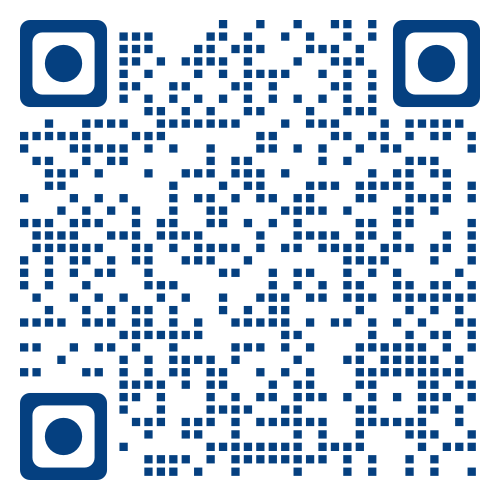
\includegraphics[height=9.6cm]{img/QRtiger.png}}; % also try shield-white.eps
\end{tikzpicture}

\end{column}

\separatorcolumn

\begin{column}{\colwidth}

  \begin{block}{Methods}

    \heading{Subjects}

  An EEG data set obtained during a Visuospatial Working Memory (VSWM) task was downloaded from OpenNeuro \citep{ds003523}; the subjects that conformed the final groups for the present analysis, mild Traumatic Brain Injury patients (mTBI, \textit{n = }27) and Healthy Controls (HC, \textit{n =}27), were matched using demographic variables and their scores in the task, thus ensuring that both groups did not differ significantly by age (\textit{p =} 0.67), sex (\textit{p =} 0.58), nor by hit ratio (\textit{p= }0.97).
    
    \heading{Procedure}

     The VSWM task (see Figure 2) was deployed using MATLAB, participants had to perform a yes-no recognition task and were asked to respond whether a location defined by a square containing a question mark (i.e. probe) had been occupied by a red dot in the preceding visual array. Participants were told to ignore the yellow dots. Altogether there were three conditions, either showing three targets or three red dots (\textit{Condition 3}), showing three targets and two distractors (\textit{Condition 3 + 2}), or showing 5 targets (\textit{Condition 5}).

    \begin{figure}
      \centering
     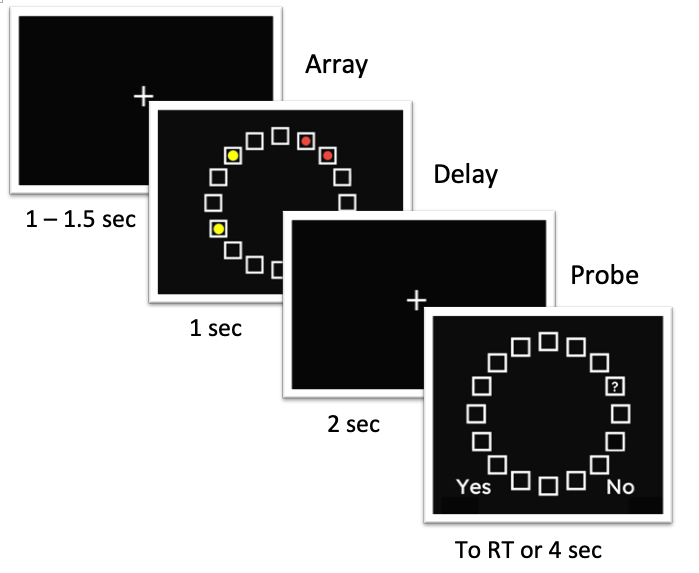
\includegraphics[width=26cm]{img/VSWM_task.png} 
      \caption{Visuospatial Working Memory (VSWM) task.}
    \end{figure}

  \heading{EEG Data}

      EEG activity was recording using a 64 channel cap and the electrodes were located according to the 10-20 system. Continuous EEG was monitored and reference to the \textit{Fz} channel and acquired at a 1000 Hz sampling rate. Total EEG set up time was in average 30 minutes, and the VSWM task included a practice block and an experimental block with 150 trials. The data of each subject that comprised the final sample was first loaded into MATLAB using EEGLab \citep{delorme2004eeglab}, then the EKG and VEOG were removed leaving only the channels that recorded brain activity.

      Following, each subject's data was decomposed by ICA using the picard algorithm \citep{ablin2018faster} and the artifact components were removed with the SASICA module \citep{chaumon2015practical}. Lastly, the data was epoched including a period from -4000 to 0 ms (i.e. 0 was the time in which the probe appeared on the screen), thus covering three memory phases (i.e. Baseline, Encoding, Retention). This data was analyzed to extract 5 frequency components from each of the scalp sites. The EEG data was labelled by group and separated as either correct or incorrect for classification purposes independently of the condition, and was exported into plain format for further processing with R \citep{R-base}. The Random Forest Algorithm was trained with 60\% of the data to build EEG classifiers of VSWM trial accuracy and diagnosis.

  \end{block}

\end{column}

\separatorcolumn

\begin{column}{\colwidth}

  \begin{block}{Results}

The first model classified Healthy Controls trials with an accuracy of 86\%; occipital $\alpha$ at encoding provided one of the highest importance values as well as parietal $\theta$ at baseline and parietal $\delta$ at encoding. The second model correctly had an accuracy of 78\% when cross-validated in mTBI data and included $\theta$ and $\beta$ bands of several channels.

Model 3 identified central-parietal $\beta$ at retention and posterior occipital $\gamma$ and $\beta$ at encoding as primary classifiers of diagnosis, providing a 98\% classification accuracy. Model 4 using the incorrect trials only, identified Central $\gamma$ at retention and baseline as primary classifiers of group belongingness. Table 1 presents a summary of the models along with the some of the variables with the larger importance in the construction of EEG classifiers for the given data set, the larger the value the more significant is for the outcome. For a complete list of the variables that resulted for each model along with the R script visit my Github page by scanning the QR code.

\begin{table}[]
\centering
\caption{Summary of Random Forest Models  with some of the variables with larger importance values}
\resizebox{\textwidth}{!}{\begin{tabular}{llllcc}
        \toprule
\multicolumn{6}{l}{\textbf{Model 1} - \textit{Healthy controls Only} - Accuracy 0.859} \\
\toprule
        & Channel & Location & Stage & Frequency & Importance \\
\midrule
        & P4    &  Parietal        & Baseline      & \theta           & 2.02            \\
        & P4    &  Parietal       & Encode       &   \delta        & 1.35           \\
        & O2    & Occipital         & Encoding      &   \alpha        &    1.13        \\
\toprule
\multicolumn{6}{l}{\textbf{Model 2} - \textit{mTBI Only} - Accuracy 0.785} \\
\midrule
        & CP2      &  Central-Parietal          &  Retention      &   \theta        &   2.32         \\
        & TP10     & Temporo-Parietal          & Retention      &   \theta        &       2.31     \\
        & TP10    & Temporo-Parietal          & Encoding     &   \alpha        &    1.72        \\
\toprule
\multicolumn{6}{l}{\textbf{Model 3} - \textit{Correct trials Only}- Accuracy 0.982}\\
\midrule
        & CP6     & Central-Parietal         & Retention       & \beta           & 5.24            \\
        & POz     & Posterior-Occipital          & Encoding       & \gamma          &  4.75          \\
        & POz      & Posterior-Occipital         & Encoding       &  \beta         &   4.66         \\
\toprule
\multicolumn{6}{l}{\textbf{Model 4} - \textit{Incorrect trials Only} - Accuracy 0.947}\\
\midrule
        & Cz        & Central         & Retention      & \gamma           &   17.4         \\
        & Cz       &   Central       & Baseline       &  \gamma         &   16.98         \\
        & CP6    &  Central-Parietal        & Retention       & \beta    & 15.16           \\
\bottomrule
\end{tabular}}
\end{table}

  \end{block}

  \begin{block}{Discussion}

    These analyses indicate that the performance in the VSMW task as well as diagnosis of the subjects based on a trial based classification approach using the Random Forest is useful for classification purposes given the high accuracy of the models; in addition, the resulting set of scalp sites and band frequencies coincide with previous findings in the working memory literature.

    For example, some experiments suggest that $\alpha$ varies as a function of memory performance, being smaller during the encoding \citep{klimesch1997eeg}. In addition, $\theta$ band activity has been associated with higher memory load \citep{boonstra2013effects}. $\gamma$ band has been associated with the integration of multi-modal sensory processes in memory tasks, and as $\theta$, it increases with higher cognitive load. Importantly $\gamma$ has been found to support short-term maintenance of information and indicates the recruitment of cognitive resources to match the demands of the cognitive task \citep{howard2003gamma}.

  \end{block}

  % \begin{block}{References}

  %   \nocite{*}
  %   \footnotesize{\bibliographystyle{apalike}\bibliography{r-references}}

  %   %\citep{delorme2004eeglab}
  %   %\cite{delorme2004eeglab}

  % \end{block}

\end{column}

\separatorcolumn
\end{columns}
\end{frame}

\end{document}
